
\section{Funcions d'agregació d'atributs}
\label{sec:model:interpolador}
\label{sec:model:agregador}


Les funcions d'agregació d'atributs s'utilitzen en la consolidació
dels buffers per tal de compactar certa informació de la sèrie
temporals. Sigui $S$ una sèrie temporal i $t_0$ i $t_f$ dos instants
de temps, una funció d'agregació d'atributs $f$ calcula una mesura que
resumeix la informació de $S$ en un interval de temps $i=[t_0,t_f]$:
\[
f: \text{sèrie temporal} \times \text{interval de temps}
\longrightarrow \text{mesura}
\]
\[
f: S=\{m_0,\ldots,m_k\} \times i=[t_0,t_f] \longrightarrow  m'
\]

\todo{vist com dues operacions}
where, generally, $m'$ results from two operations on the time series: (i) a time subseries selection $S'$ depending on the consolidating interval, for example $S' = S[t_0,t_f]$, and (ii) an aggregation over this time subseries  $m' = \agg(S',m_i a)$ with $a: m_i \times m\rightarrow m''$. \todo{mirar bé la sintaxi agg}

Atès que hi ha maneres diferents de resumir la informació d'una sèrie
temporal, hi ha diferents funcions d'agregació d'atributs. Per
exemple, es poden calcular estadístics de la sèrie temporal, com el
valor màxim o la mitjana, o aplicar operacions de processament digital
del senyal, com fan \textcite{zhang11}.  La representació de les
sèries temporals (v.\ sec.~\ref{sec:model:repr}) pot afectar els
càlculs que es fan en l'agregació i l'agregació pot ser utilitzada per
a tractar algunes de les patologies de les sèries temporals
(v.\ sec.~\ref{sec:sgst:patologies}).


Així doncs, es poden definir una enorme varietat de funcions
d'agregació d'atributs i no hi ha cap assumpció global que es pugui
fer. Com a conseqüència, els \gls{SGSTM} han de donar llibertat als usuaris
per a definir funcions d'agregació d'atributs personalitzades.

A continuació descrivim algunes interpretacions possibles que es poden
fer de les funcions d'agregació, tant pel que fa al càlcul de
l'instant de temps de consolidació com pel que fa al càlcul amb
representació de sèries temporals, i descrivim com utilitzar les
funcions d'agregació per a tractar i validar dades desconegudes en les
sèries temporals.



\todo{explicar dibuix i situar al lloc correcte}

    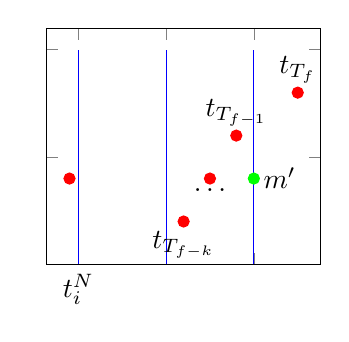
\begin{tikzpicture}
        \begin{axis}[
          % width=10cm,
          scale only axis, height=3cm,
          ymin = 0,
          yticklabels= {},
          xticklabels={$\ldots$,$t_{i-1}^N$,$t_i^N$},
          ]
          \addplot[ycomb,blue] coordinates {
            (20,10)
            (30,10)
            (40,10)
          }; 
          
          \addplot[only marks,mark=*,red] coordinates {
            (19,4)
            (32,2)
            (35,4)
            (38,6)
            (45,8)
          };
          
          \addplot[only marks,mark=*,green] coordinates {
            (40,4)
          };
          
          
          \node[below] at (axis cs:32,2) {$t_{T_{f-k}}$};
          \node[below] at (axis cs:35,4) {$\ldots$};
          \node[above] at (axis cs:38,6) {$t_{T_{f-1}}$};
          \node[above] at (axis cs:45,8) {$t_{T_f}$};
          \node[right] at (axis cs:40,4) {$m'$};
        \end{axis}
      \end{tikzpicture}



\subsection{Interpretació de l'agregació}

L'agregació d'una sèrie temporal es pot dur a terme en forma discreta
o en forma contínua.  En la forma discreta es tracta la sèrie temporal
com a conjunt o seqüència de mesures, és per tant semblant a la
representació amb funcions parcials, i en canvi en la forma contínua
es tracta la sèrie temporal com a funció temporal, per tant s'utilitza
una representació contínua de la sèrie temporal.

De forma general podem definir patrons per a les funcions d'agregació
d'atributs en forma discreta i en forma contínua. Tot i així, en
ambdós casos l'instant de temps d'agregació resultant $T(m')$ no queda
definit sinó que es pot interpretar per a cada cas, la qual cosa es detalla
més endavant.


En primer lloc, les funcions d'agregació amb forma discreta (d)
treballen amb operadors de conjunts sobre la sèrie temporal. En els
patrons d'aquestes funcions, a banda del temps d'agregació resultant
$T(m')$, l'interval de consolidació $i=[t_0,t_f]$ també es pot
interpretar per a cada cas. Així sigui $S$ la sèrie original, el
resultat es pot calcular sobre una subsèrie amb interval obert
$S'=S(t_0,t_f)$, tancat $S'=S(t_0,t_f]$, semiobert $S'=S(t_0,t_f]$ o
$S'=S[t_0,t_f)$, o altres combinacions com per exemple tenir
desfasaments $S'=S[t_0-d,t_f-d]$ a on $d$ és una durada. A continuació
es mostren alguns exemples de patrons per a resumir determinats
atributs:
\begin{itemize}
\item màxim$^d$: $S \times i \mapsto m'$ a on $V(m') = \max_{\forall m
    \in S'}(V(m))$. Resumeix $S'$ amb el màxim dels valors de les
  mesures.

  % Amb operacions de \gls{SGST} es pot calcular amb
  % $V\big(\glssymbol{not:sgst:aggregate}(S',(0,\infty), (t^i,v^i)
  % \times (t,v) \mapsto [(0,v^i) \text{ if } v < v^i \wedge
  % v^i\neq\infty \text{ else } (0,v) ])\big)$.

\item darrer$^d$: $S \times i \mapsto m'$ a on $V(m') =
  \max(S')$. Resumeix $S'$ amb el valor de la mesura màxima.
\item mitjana aritmètica$^d$: $S \times i \mapsto m'$ a on $V(m') =
  \frac{1}{|S'|} \sum\limits_{\forall m\in S'} V(m)$, o bé $V(m') =
  \glssymbol{not:sgst:mitjanav}(S')$ segons definit al model de
  \gls{SGST}. Resumeix $S'$ amb la mitjana dels valors de les mesures.
\end{itemize}


En segon lloc, les funcions d'agregació amb forma contínua (c)
treballen amb operadors de funció temporal sobre la sèrie temporal.
En els patrons d'aquestes funcions es treballa sobre una funció
contínua $S(t)$, que a cada cas serà una funció de representació
concreta i el temps d'agregació resultant $T(m')$ serà interpretat
coherentment.  A continuació es mostren alguns exemples de patrons per
a resumir determinats atributs, sigui el temps continu per tot el
domini de temps $t\in T$:
\begin{itemize}
\item màxim$^c$: $S \times i \mapsto m'$ a on $V(m') = \max_{\forall t
    \in [t_0,t_f]}(S(t))$. Resumeix $S$ amb el màxim dels valors de
  les mesures a l'interval $i$.
\item darrer$^c$: $S \times i \mapsto m'$ a on $V(m') =
  S(t_f)$. Resumeix $S$ amb el valor del darrer instant de temps de
  l'interval $i$.

\item mitjana$^c$: $S \times i \mapsto m'$ a on $V(m') =
  \frac{1}{t_f-t_0} \int_{t_0}^{t_f} S(t)dt$. Resumeix $S$ amb la
  \emph{mitjana de la funció} \parencite{weisstein:averagefunction} a
  l'interval $i$.  
  % Explicació:
  % If $f$ is continuous on a closed interval $[a,b]$, then there is at least one number $x^*$ in $[a,b]$ such that
  % $$
  % \int_a^b f(x)dx = f(x^*)(b-a)
  % $$

  % The average value of the function ($\bar f$)  on this interval is then given by  $f(x^*)$.
  % $S(t)$ ha de ser contínua en l'interval $i$.
\end{itemize}


A continuació s'exemplifiquen algunes interpretacions possibles de
l'instant de temps resultant i de les representacions per a aquests
patrons. 

Per al cas de funcions d'agregació amb forma discreta es poden
interpretar des de les representacions parcials i per tant
implementar-les amb operadors de conjunts o de seqüències.  
Per al cas de funcions d'agregació amb forma contínua, els patrons
estan definits com a problemes d'anàlisi numèric però a cada cas
$S(t)$ és una funció que prové d'un conjunt de mesures i podem
expressar els operadors segons el model de \gls{SGST} descrit amb matemàtica
discreta. Així doncs, les funcions d'agregació acaben tenint forma
discreta tot i que a l'hora d'interpretar-les cal observar si el patró
té origen continu o discret.




\subsubsection{Temps d'agregació resultant}

L'objectiu de les funcions d'agregació d'atributs és determinar un
instant de temps $T(m')$ i un valor $V(m')$. Aquest càlcul del temps i
del valor es pot realitzar al mateix temps però també pot ser
independent. Així normalment el temps resultant serà independent i
valdrà $T(m')=t_f$ per estar d'acord amb l'operació de consolidació
del buffer i no provocar desfasament de la subsèrie resolució
(v.~\autoref{def:sgstm:desdsamentR}), però en alguns casos aquest
$T(m')$ serà dependent del valor calculat o estarà subjecte a una
interpretació adient com és el cas per les representacions a
l'apartat següent.


Un exemple de funció d'agregació on temps i valor són dependents és
una que retorni la primera mesura que troba, $\operatorname{primera}:
S \times i \mapsto m'$ a on $m' = \min(S[t_0,t_f))$ i llavors el temps
resultant pot ser $t_0 \leq T(m') < t_f$. En aquest cas la sèrie
temporal resultant no és regular.


Un exemple de funció d'agregació on temps i valor són independents i
on la subsèrie resolució resultant és regular però amb desfasament, és
una funció que fa la mitjana amb un desfasament de 5 unitats de temps.
$\operatorname{mitjanad5}: S \times i \mapsto m'$ a on $V(m')=
\glssymbol{not:sgst:mitjanav}(S[t_0-5,t_f-5))$ i $T(m')=t_f-5$. La
funció d'agregació $\operatorname{mitjanad5}$ s'ha utilitzat
anteriorment a l'\autoref{ex:model:bdm-desfasaments}.

%De què pot servir la mitjanad5? per calcular mitjanes centrades? estem fent una interpolació sobre la representació centrada en l'interval de la sèrie temporal?


%mitjana mòbil, MM
%moving average, MA




\subsubsection{Agregació amb representació}

La varietat de funcions de representació per les sèries temporals
indueix a una varietat de funcions d'agregació per a un mateix
atribut. Per exemple, la funció d'agregació per l'atribut de màxim$^c$
dóna com a resultat valors diferents si es considera una representació
lineal o una representació a trossos constant. A continuació mostrem
la interpretació dels patrons continus definits anteriorment per a
dues representacions: la delta i la ZOHE.

Per a les funcions d'agregació delta interpretem el temps d'agregació
resultant centrat en l'interval $T(m')=\frac{t_f+t_0}{2}$, tot i que
en aquest cas altres interpretacions també es podrien considerar com
per exemple $T(m')=t_f$. Així de forma general podem definir les
funcions d'agregació d'atributs amb representació delta $f^\delta\in
f$ com $f^\delta: S \times [t_0,t_f] \mapsto m'$ a on
$m'=(\frac{t_f+t_0}{2},v')$ i el valor resultant depèn de l'atribut
que es vulgui resumir calculat en l'interval temporal delta
$S'=S[t_0,t_f]^\delta$:

\todo{la delta ha canviat el nom a DD}

\begin{itemize}
\item \glssymboldef{not:sgstm:maxdd}\todo{canviar} màxim$^\delta$: $S
  \times i \mapsto m'$ a on $V(m') = \max\big(0,\max_{\forall m \in
    S'}(V(m))\big)$ i $T(m')=\frac{t_f+t_0}{2}$. \todo{símbol declarat
    a la notació} \todo{s'hauria de dir que $\max(V(m))$ és el mateix
    que $\glssymbol{not:sgst:maxv}(S')$}

\item darrer$^\delta$: $S \times i \mapsto m'$ a on $V(m') =
  \max(S')$ i $T(m')=\frac{t_f+t_0}{2}$.

\item \glssymboldef{not:sgstm:mitjanadd}\todo{canviar}
  mitjana$^\delta$: $S \times i \mapsto m'$ a on $V(m') =
  \frac{1}{t_f-t_0}\sum\limits_{\forall m \in S'} V(m)$ i
  $T(m')=\frac{t_f+t_0}{2}$. Nota: la funció delta té la propietat
  fonamental $\int \delta(t)dt = 1$. \todo{símbol declarat a la
    notació} \todo{relació amb  $\glssymbol{not:sgst:mitjanav}(S')?$}
\end{itemize}



Per a les funcions d'agregació ZOHE interpretem sempre el temps
d'agregació resultant com $T(m')=t_f$, atès que la representació ZOHE
es defineix amb funcions graó contínues per l'esquerra. Així de forma
general podem definir les funcions d'agregació d'atributs amb
representació ZOHE $f^{\text{ZOHE}}\in f$ com $f^{\text{ZOHE}}: S
\times [t_0,t_f] \mapsto m'$ a on $m'=(t_f,v')$ i el valor resultant
depèn de l'atribut que es vulgui resumir calculat en l'interval
temporal ZOHE $S'=S[t_0,t_f]^\text{ZOHE}$:
\begin{itemize}
\item màxim$^\text{ZOHE}$: $S \times i \mapsto m'$ a on $V(m') = \max_{\forall m
    \in S'}(V(m))$ i $T(m')=t_f$.

\item darrer$^\text{ZOHE}$: $S \times i \mapsto m'$ a on $V(m') =
  \max(S')$ i $T(m')=t_f$.

\item \todo{declarar a la notació}\todo{potser estaria bé fer-ne un dibuix} mitjana$^\text{ZOHE}$: $S \times i \mapsto m'$ a on $V(m') =
  \frac{1}{t_f-t_0} \big[ (T(o)-t_0)V(o) +
  \sum\limits_{\forall m \in S''}( T(m)- T(\glssymbol{not:sgst:prev}_S
  m) )V(m) \big]$, $o=\min(S')$, $S''= S' - \{o\}$ i
  $T(m')=T_f$. 
% \[
%   \begin{split}
%   V(m')  = & \frac{1}{T_f-T_0} 
%   \big[ (T(o)-T_0)V(o) -( T(n)-T_f)V(n) \\
%     & {}+\sum\limits_{\forall m \in S''}( T(m)- T(\prev_S m) )V(m) \big]   
%    \end{split}
%   \]
% Nota: s'aplica la definició $0 \times \infty = 0$ tal com es fa habitualment a la teoria de mesura, \cite{wiki:extendedreal}.
\end{itemize}

\textcite{rrdtool} utilitza a RRDtool una funció d'agregació com la
mitjana$^\text{ZOHE}$ per a resumir la informació conservant el
comptatge total si les sèries temporals mesurades tenen trets
semàntics de comptador i són en forma de velocitat; així aquesta
agregació es pot veure com una consolidació que conserva l'àrea del
senyal original.


En conclusió, per una banda alguns exemples mostrats de patrons
continus tenen un patró semblant a algunes funcions d'agregació en
forma discreta, per exemple el màxim i el darrer, i en certa manera
només es diferencien en la interpretació de l'interval on s'ha de
resumir la sèrie temporal. Per altra banda, altres exemples són molt
diferents, com és el cas de la mitjana$^\text{ZOHE}$ que té una
interpretació més complexa que la mitjana aritmètica$^d$. En aquest
cas també es podria dissenyar una mitjana aritmètica en l'interval
temporal ZOHE, és a dir una mitjana simple sense tenir en compte els
pesos del temps
$\glssymbol{not:sgst:mitjanav}(S[t_0,t_f]^\text{ZOHE})$. Però llavors
s'hauria d'interpretar quin patró continu d'origen li correspondria,
altrament aquesta operació d'agregació podria no tenir sentit real.



% Notes:

% * Quan una sèrie temporal és regular, l'intepolador mitjana aritmètica i l'interpolador àrea valen el mateix en l'interval $(T_o,n\delta]$.




\subsection{Tractament i validació de dades}

Les funcions d'agregació d'atributs poden cooperar en els processos de
validació i tractament de dades En les patologies de les sèries
temporals (v.\ apartat~\ref{sec:sgst:patologies}) s'ha descrit el
problema de les dades desconegudes, les funcions d'agregació poden
marcar o tractar les dades desconegudes:
\begin{itemize}
\item Marcar dades com a desconegudes. És a dir determinar quan el
  resultat d'una agregació ha de ser desconegut perquè la sèrie
  temporal avaluada pateix una de les causes descrites: valors fora de
  rang, temps de termini excedit, etc.

\item Tractar dades que són desconegudes, ja sigui perquè d'origen són
  desconegudes o perquè les hem marcat abans com a desconegudes.
  Si una funció d'agregació rep valor que són desconeguts, des d'un
  punt de vista estricte el resultat de l'agregació ha de ser
  desconegut. No obstant això, es poden aplicar operacions que tractin
  aquest valors desconeguts: reconstrucció del senyal, ignorar els
  valors desconeguts, etc.
\end{itemize}

 
A continuació definim el procés que fan les funcions d'agregació per a
ambdós casos. Utilitzem el nombres reals projectius
\glssymbol{not:R*} amb els quals representem el valor desconegut
amb l'element infinit ($\infty$), segons la
\autoref{def:model:mesura_valor_indefinit} de mesura de valor indefinit.


Una funció d'agregació d'atributs $f^u \in f$ que tracti dades
desconegudes és aquella que pot calcular un resultat quan la sèrie
temporal original conté valors desconeguts
\[
f^u: S \times i \mapsto m' \text{ a on } \exists m \in S: V(m)=\infty
\]

Per exemple, podem redefinir la funció d'agregació mitjana$^c$ en una
$\operatorname{mitjana}^{cu}$ que sigui capaç de tractar valors
desconeguts conservant l'àrea coneguda; és a dir, l'àrea total
coneguda quedarà escampada en l'interval de consolidació.
\begin{gather*}
  \operatorname{mitjana}^{cu}: S \times i \mapsto m' \text{ a on }\\
  V(m') = \frac{1}{t_f-t_0}\int_{t_0}^{t_f} S^u(t)dt \text{ i }
  S^u(t)=
  \begin{cases}
    0 &\text{si }  S(t)=\infty\\
    S(t) & \text{altrament }
  \end{cases}
\end{gather*}



Una funció d'agregació d'atributs $f^{mu} \in f$ que marqui
dades desconegudes és aquella que pot retornar una mesura de valor
indefinit com a resultat.
\[
f^{mu}: S \times i \mapsto m' \text{ a on } V(m')\in \glssymbol{not:R*}
\]


Per exemple, podem definir una funció d'agregació d'atribut
màxim$^{\delta S2}$ que, basat la funció màxim$^\delta$, retorni valor desconegut
si hi ha un a mesura amb el valor més gran que 2; és a dir establim un
límit superior de 2 (S2). 
\begin{gather*}
  \operatorname{m\grave{a}xim}^{\delta S2}: S \times i \mapsto m' \text{ a on }\\
  m' = \begin{cases}
    (T(m''),\infty) &\text{si }  \exists m\in S[t_0,t_f]: V(m)>2\\
    m'' & \text{altrament }
  \end{cases} \text{ i } m''= \operatorname{m\grave{a}xim}^\delta(S,i)
\end{gather*}






%Per exemple definim un termini, si les dades estan més espaiades que 2 es marca com a desconeguda
% Sigui $S=\{m_0,\ldots,m_k\}$ una sèrie temporal i $H$ un termini de temps, una mesura $m_i=(v_i,t_i)\in S$ és desconeguda si, donada la mesura anterior $m_{i-1}=(v_{i-1},t_{i-1})$, $t_i - t_{i-1} > H$.    





% Sigui $S=\{m_0,\ldots,m_k\}$ una sèrie temporal, $f$ un interpolador, $i=[T_0,T_f]$ un interval de temps i $\alpha$ un llindar, la mesura de consolidació calculada per l'interpolador $f$ és desconeguda ssi  
% \[
% \frac{t_d }{T_f - T_0} > \alpha :
% \]
% \[
% :t_d = t_{d0} + t_{df} + \sum\limits_{i=1}^{k-1}(t_i-t_{i-1}) : v_k = 'desconegut':
% \]
% \[
% : t_{d0} = \left\{\begin{array}{l} t_0-T_0 \text{ si } v_0 = 'desconegut' \\ 0\end{array}\right. ,
% t_{df} = \left\{\begin{array}{l} T_f-t_{k-1} \text{ si } v_k = 'desconegut' \\ 0\end{array}\right. :
% \]
% \[
% :k=|S|-1,(v_k,t_k)=m_k\in S' :S'= S_{T_0:T_f} \cup \{min(S_{T_f:\infty})\}
% \]



%operacions amb nan de octave i matlab
%http://biosig-consulting.com/matlab/NaN/
% The NaN-toolbox v2.0: A statistics and machine learning toolbox for Octave and Matlab
% for data with and w/o MISSING VALUES encoded as NaN's.











%%% Local Variables:
%%% TeX-master: "main"
%%% End:
% LocalWords: buffer buffers ZOHE





